\chapter{Set-Up of Experiment}
    To perform the experiment the items shown in \cref{fig:setup} are needed.
    %
    \begin{figure}[H]
        \centering
        % \begin{framed}
            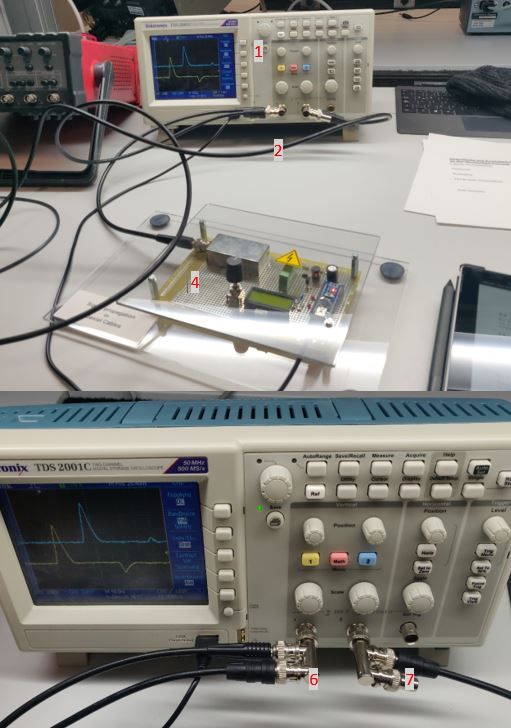
\includegraphics[width=.7\textwidth]{aufbau/setup_num.JPG}
        % \end{framed}
        %\includegraphics[width=12cm]{} % insert image (incl. numbering)
        \caption{Components needed for the experiment. 1. Oscilloscope, 2. Coaxial cables in various lengths, 3. Circuit board, 4. T-piece, \SI{50}{\ohm} transmission line terminator.}
        \label{fig:setup}
    \end{figure}
    %
    A detailed overview of the circuit board (position 3 in \cref{fig:setup}) will give \cref{fig:circuit_board} below.
    %
    \begin{figure}[H]
        \centering
        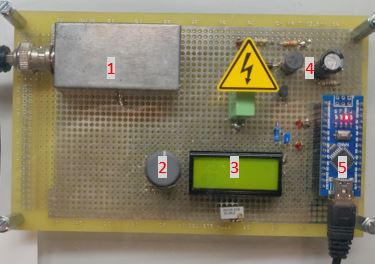
\includegraphics[width=.7\textwidth]{aufbau/circuit_board_num.JPG}
        \caption{Detailed view on the circuit board. 1. APG, 2. Potentiometer to adjust the voltage fed into the APG, 3. LC-Display to monitor
        the the BC's output voltage, 4. BC-circuit, 5. \micro-controller and PSU}
        \label{fig:circuit_board}
    \end{figure}
    %